\documentclass[conference]{IEEEtran}

\usepackage{cite}
\usepackage{amsmath,amssymb}
\usepackage{graphicx}
\usepackage{booktabs}
\usepackage{array}
\usepackage{url}
\usepackage{algorithm}
\usepackage{algorithmic}
\usepackage{multirow}
\usepackage[hidelinks]{hyperref}

\graphicspath{{figures/}{figures/screenshots/}}

\begin{document}

\title{HeartCareAI: A Web-Based Machine Learning System for Heart Disease Screening Support}

\author{
\IEEEauthorblockN{Jayant Malik}
\IEEEauthorblockA{\textit{School of Computing and}\\
\textit{Artificial Intelligence}\\
\textit{Lovely Professional University}\\
Phagwara, Punjab, India\\
jayantmalik743malik@gmail.com}
\and
\IEEEauthorblockN{Vansh Vaid}
\IEEEauthorblockA{\textit{School of Computing and}\\
\textit{Artificial Intelligence}\\
\textit{Lovely Professional University}\\
Phagwara, Punjab, India\\
vaidvansh6@gmail.com}
\and
\IEEEauthorblockN{Nayanava Mal}
\IEEEauthorblockA{\textit{School of Computing and}\\
\textit{Artificial Intelligence}\\
\textit{Lovely Professional University}\\
Phagwara, Punjab, India\\
nayanava701@gmail.com}
}

\maketitle

\begin{abstract}
Cardiovascular disease creates a continuing need for tools that encourage early risk awareness without replacing clinical judgement. This paper describes HeartCareAI, a Flask-based screening support application that moves beyond a standalone prediction script by joining model inference with patient, doctor, and administrator workflows. The application validates clinical inputs, loads a versioned model artifact, produces calibrated probability estimates, records the threshold used for interpretation, stores prediction history, renders reports, presents exploratory charts, and provides retrieval-based chatbot assistance from local project knowledge files. The training workflow uses 8,565 cleaned records, 15 model features, engineered interaction variables, train/validation/test separation, and comparative evaluation of Random Forest, XGBoost, Support Vector Machine, and Logistic Regression models. In the project report, the Random Forest model produced the strongest reported result with 99.71\% accuracy, 99.88\% precision, 99.53\% recall, 99.70\% F1-score, and 100.00\% AUC-ROC. These results are presented as dataset-bound project findings rather than evidence of clinical readiness. HeartCareAI is intended for educational screening support and decision awareness; it is not a diagnostic medical device. Broader validation, bias review, security hardening, and clinician-centered testing are necessary before any deployment in real healthcare settings.
\end{abstract}

\begin{IEEEkeywords}
heart disease screening, machine learning, Flask, clinical decision support, calibrated prediction, Random Forest, healthcare web application
\end{IEEEkeywords}

\section{Introduction}
Cardiovascular disease remains a major cause of mortality and long-term illness, making earlier recognition of possible risk an important public health objective \cite{who_cvd}. A software screening tool cannot decide whether a patient has heart disease, yet it can help organize risk-related measurements and make users more aware of when a professional consultation may be appropriate. Heart disease prediction is a natural candidate for structured machine learning because many commonly collected indicators, including age, chest pain type, resting blood pressure, cholesterol, electrocardiographic findings, maximum heart rate, and exercise-induced angina, can interact in ways that are difficult to summarize manually.

The central challenge is not only training a classifier, but also shaping the classifier into a responsible application workflow. In a deployed-style system, the live form must respect the same feature schema used during training, invalid physiological values must be rejected, model versions should be traceable, and the output should communicate uncertainty rather than hide it behind a bare positive or negative label. This project therefore treats the model as one component in a larger screening-support service.

HeartCareAI was built around that service view. It combines a heart disease prediction pipeline with a Flask web interface where patients can submit screening data, doctors can review patient-related records, and administrators can monitor system activity. The application also includes prediction history, report pages, exploratory data analysis charts, and a local retrieval chatbot that answers questions from project-specific guide files. As a result, the work documents both the predictive layer and the application layer that carries the prediction to users.

The main contributions of this project are:
\begin{itemize}
    \item a Flask-based role-aware screening platform for patient, doctor, and administrator workflows;
    \item a machine learning pipeline with train/validation/test separation and model comparison;
    \item calibrated probability output with threshold-based interpretation rather than only a hard class label;
    \item integrated reports, model visualizations, and prediction history views;
    \item a retrieval-based chatbot that provides grounded help without presenting itself as a clinician.
\end{itemize}

\section{Related Work}
Conventional cardiovascular risk assessment depends on clinical history, physical measurements, laboratory values, symptoms, and physician interpretation. These approaches are trusted partly because clinicians understand the inputs and the reasoning process. Data-driven models offer a different advantage: they can detect nonlinear combinations of tabular variables, although that flexibility also increases the need for careful validation and cautious communication. For student and research prototypes, the most useful comparison is often between interpretable baselines and stronger nonlinear models.

Random Forests aggregate many decision trees and are useful for tabular biomedical classification because they can capture interactions without requiring every rule to be manually specified \cite{breiman_rf}. XGBoost uses gradient-boosted trees and has become a common high-performing option for structured data tasks \cite{chen_xgboost}. Support Vector Machines provide a margin-based classifier, while Logistic Regression remains valuable as a simpler binary baseline. HeartCareAI follows this comparative pattern and uses the Python machine learning ecosystem, including scikit-learn-style preprocessing, evaluation, and pipeline organization \cite{scikit_learn}.

Clinical machine learning systems also require more than discrimination metrics. Reporting guidance such as TRIPOD emphasizes transparent model development and validation \cite{tripod}. Calibration is important because a probability should correspond meaningfully to observed event frequency, especially when a prediction is presented to users rather than hidden inside a backend decision rule. In health applications, model performance should also be checked across populations, institutions, and time, because a model that performs well on one dataset may not generalize to a different clinical environment.

HeartCareAI is positioned as a deployment-oriented student research system. Its goal is not to claim clinical approval, but to demonstrate how a predictive model can be wrapped with validation, user roles, report generation, and cautious risk communication.

\section{System Overview}
HeartCareAI is organized as a layered Flask application. The browser interface presents forms, dashboards, reports, and chart views. Flask routes coordinate authentication, role-specific access, and page submission, while the prediction service handles the model-facing work. During inference, the service loads the promoted model bundle, checks the submitted fields against the expected schema, constructs engineered features, estimates a calibrated probability, applies the configured threshold, and returns a screening interpretation. The database stores prediction records with model metadata so that later reports can identify the model name, version, threshold, and probability behind a displayed result.

\begin{figure}[!t]
    \centering
    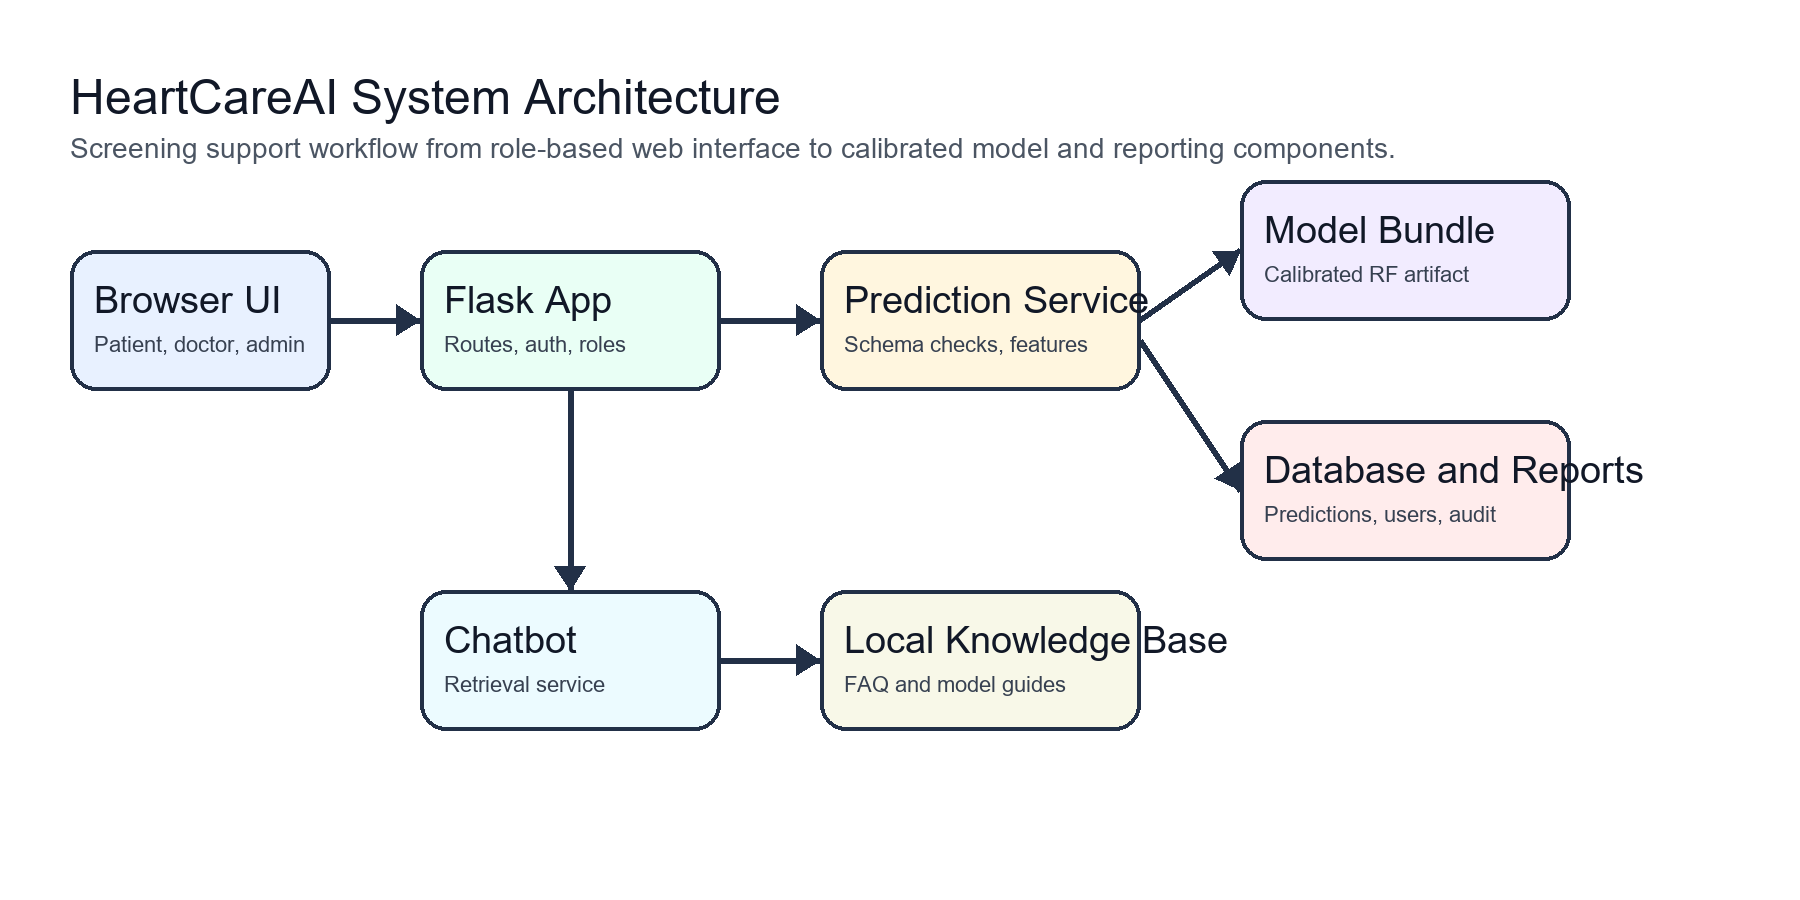
\includegraphics[width=\linewidth]{architecture.png}
    \caption{HeartCareAI system architecture. The web interface communicates with Flask routes, the prediction service, model artifact, database/reporting layer, and a retrieval-based chatbot backed by local knowledge files.}
    \label{fig:architecture}
\end{figure}

The administrator workflow supports user, doctor, patient, and prediction monitoring. The doctor workflow supports patient review and detail pages. The patient workflow supports registration, prediction entry, result review, and historical report access. The chatbot module uses local documents such as feature guides, model guides, prediction guides, and frequently asked questions. If a hosted language model key is configured, the chatbot can synthesize grounded answers; otherwise it remains a retrieval-only assistant.

\section{Dataset and Preprocessing}
The dataset used in the project contains 8,565 records after cleaning. The model receives 15 inputs: thirteen direct clinical or demographic variables and two engineered variables. The engineered variables are the blood-pressure-to-cholesterol ratio and an age-cholesterol interaction, both included to expose simple combined patterns to the classifier. The final target distribution is close to balanced, with 4,906 records labeled as no disease and 4,891 records labeled as disease.

\begin{table}[!t]
\caption{Dataset Summary}
\label{tab:dataset}
\centering
\begin{tabular}{lr}
\toprule
\textbf{Property} & \textbf{Value} \\
\midrule
Total cleaned rows & 8,565 \\
Model features & 15 \\
Training samples & 5,139 \\
Validation samples & 1,713 \\
Test samples & 1,713 \\
No-disease records & 4,906 \\
Disease records & 4,891 \\
Class balance ratio & 0.997 \\
\bottomrule
\end{tabular}
\end{table}

Preprocessing standardized column names, removed outliers using the interquartile range method, created engineered variables, and saved the feature schema used by the trained artifact. The schema step is important because the web form does not operate in the same environment as the training script. If a live request changes field names, ordering, or value types, the model may receive an invalid representation even when the form appears complete to the user.

\begin{table}[!t]
\caption{Clinical Input Validation Ranges}
\label{tab:ranges}
\centering
\begin{tabular}{lll}
\toprule
\textbf{Feature} & \textbf{Range} & \textbf{Unit} \\
\midrule
Age & 18--100 & years \\
Resting blood pressure & 80--200 & mmHg \\
Cholesterol & 100--400 & mg/dL \\
Maximum heart rate & 60--220 & bpm \\
ST depression & 0--10 & numeric \\
\bottomrule
\end{tabular}
\end{table}

\section{Methodology}
The modeling workflow starts from the cleaned table and separates records into training, validation, and test partitions. Candidate classifiers are tuned and compared using validation behavior rather than only training accuracy. After model selection, the promoted estimator is calibrated so the output can be treated as a probability estimate instead of only a relative score. HeartCareAI then applies a threshold to convert that probability into a screening interpretation and saves the model artifact with schema and metric metadata.

\begin{algorithm}[!t]
\caption{HeartCareAI Training and Prediction Workflow}
\label{alg:workflow}
\begin{algorithmic}[1]
\STATE Load cleaned heart disease dataset.
\STATE Apply validation ranges and remove invalid records.
\STATE Create engineered features.
\STATE Split data into training, validation, and test sets.
\STATE Train candidate classifiers with cross-validation.
\STATE Tune hyperparameters and compare validation behavior.
\STATE Calibrate probability outputs for the promoted model.
\STATE Save model bundle, schema, metrics, and version metadata.
\STATE For live prediction, validate form input against schema.
\STATE Generate engineered features and estimate probability.
\STATE Apply threshold and store prediction with model version.
\end{algorithmic}
\end{algorithm}

The application report identifies Random Forest as the best-performing model in the reported comparison. Tree ensembles are suitable for this type of structured data because they can model nonlinear interactions without requiring manual transformation of every feature. Logistic Regression remains useful as a baseline because it exposes the contrast between a simpler linear model and more flexible classifiers.

\section{Implementation}
The codebase is arranged as a modular Flask project. Separate blueprints handle authentication, main pages, prediction, reporting, chatbot interaction, doctor views, and administrator views. This separation keeps the user interface routes from becoming a single large controller and makes the role-specific pages easier to maintain. The database stores users, doctors, patients, and prediction-related records, allowing the application to support patient history and administrative review.

The prediction layer is deliberately separated from the route layer. Model loading, input validation, schema checks, feature construction, probability estimation, threshold application, and explanation metadata are handled in a service component rather than being embedded in HTML templates. For each prediction, the application can store the estimated probability, threshold, model name, model version, confidence label, explanation payload, and input audit information. This makes a prediction more reviewable than a single stored class label.

Reports and visualization pages help users inspect both individual results and model development artifacts. The chatbot uses local retrieval from project knowledge files, which reduces the risk of unsupported free-form medical claims. The chatbot is intended to explain application features and model behavior in plain language, not to provide diagnosis or treatment instructions.

\section{Results and Evaluation}
Table~\ref{tab:comparison} presents the model comparison values from the project report. The Random Forest and XGBoost models performed similarly on the reported metrics, while SVM also produced strong discrimination. Logistic Regression trailed the nonlinear models but remained a useful baseline.

\begin{table}[!t]
\caption{Model Comparison from the HeartCareAI Project Report}
\label{tab:comparison}
\centering
\scriptsize
\resizebox{\linewidth}{!}{%
\begin{tabular}{lrrrrrr}
\toprule
\textbf{Model} & \textbf{Accuracy} & \textbf{Precision} & \textbf{Recall} & \textbf{F1-score} & \textbf{AUC-ROC} & \textbf{Val. Acc.} \\
\midrule
Random Forest & 99.71 & 99.88 & 99.53 & 99.70 & 100.00 & 99.82 \\
XGBoost & 99.71 & 99.88 & 99.53 & 99.70 & 100.00 & 99.65 \\
SVM & 99.59 & 99.29 & 99.88 & 99.59 & 100.00 & 99.59 \\
Logistic Regression & 81.09 & 77.43 & 86.97 & 81.92 & 88.68 & 79.68 \\
\bottomrule
\end{tabular}
}
\end{table}

For the best reported Random Forest result, the confusion matrix contained 868 true negatives, 1 false positive, 4 false negatives, and 840 true positives. This indicates very high performance on the available evaluation split. Because these scores are unusually strong for a medical prediction task, they should be treated as project-level evidence rather than proof of clinical generalization. A separate promoted model artifact in the application also records calibrated threshold-based metrics, emphasizing sensitivity and probability quality for operational screening behavior.

\begin{figure}[!t]
    \centering
    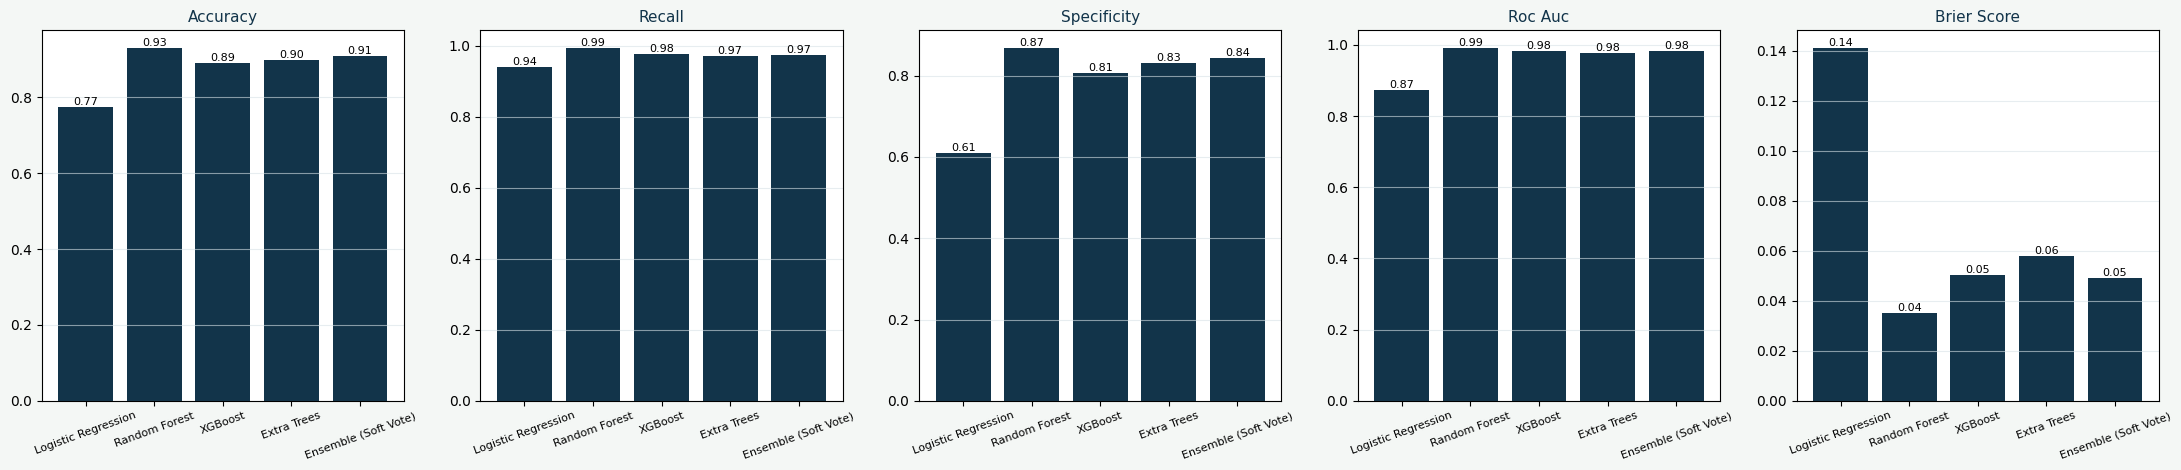
\includegraphics[width=\linewidth]{model_comparison.png}
    \caption{Model comparison chart generated from the HeartCareAI training pipeline.}
    \label{fig:modelcomparison}
\end{figure}

\begin{figure}[!t]
    \centering
    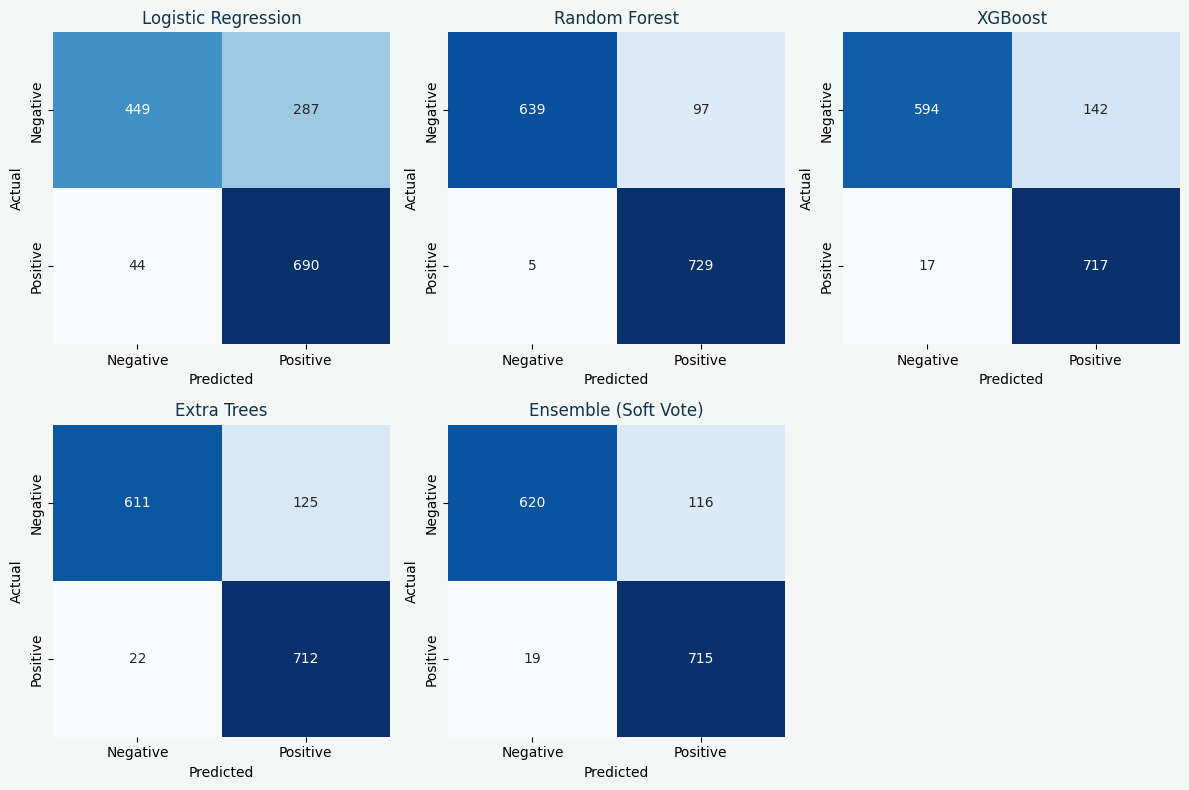
\includegraphics[width=\linewidth]{confusion_matrices.png}
    \caption{Confusion matrix visualization for evaluated classifiers.}
    \label{fig:confusion}
\end{figure}

\begin{figure}[!t]
    \centering
    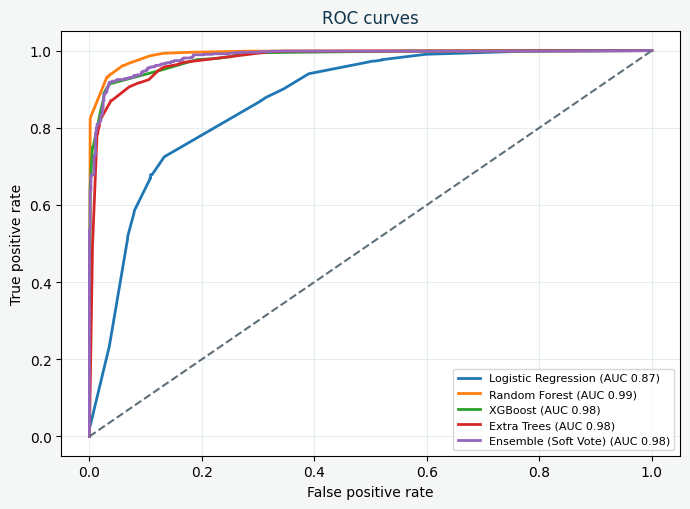
\includegraphics[width=\linewidth]{roc_curves.png}
    \caption{ROC curve visualization used to compare model discrimination.}
    \label{fig:roc}
\end{figure}

\begin{figure}[!t]
    \centering
    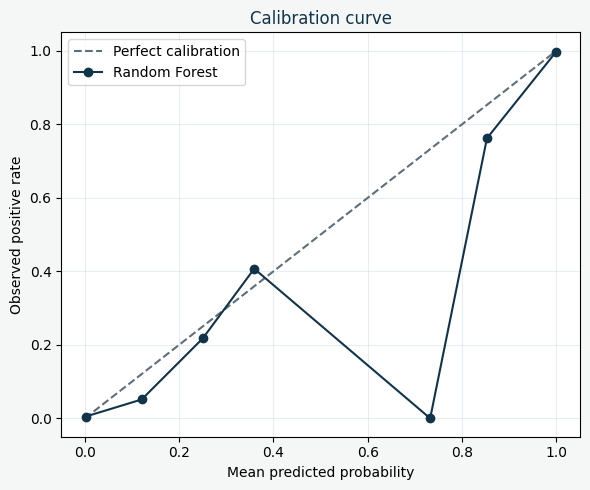
\includegraphics[width=\linewidth]{calibration_curve.png}
    \caption{Calibration curve used to inspect probability reliability.}
    \label{fig:calibration}
\end{figure}

\section{User Interface and Workflow}
The HeartCareAI interface is organized around user roles instead of presenting every feature on one page. A patient can register, sign in, submit screening indicators, view the generated result, and return to earlier predictions. A doctor can inspect patient-related information and prediction details, while an administrator can review users, doctors, patients, and prediction activity. This role-aware structure gives the project a workflow closer to a practical screening tool than a notebook export.

The prediction form collects the clinical variables required by the model and sends them through the same validation contract used during training. The result page presents a calibrated probability and threshold-based interpretation. This is preferable to displaying only a class label, because a probability can communicate risk gradation more clearly. The report view helps preserve the prediction context for later review.

\begin{figure}[!t]
    \centering
    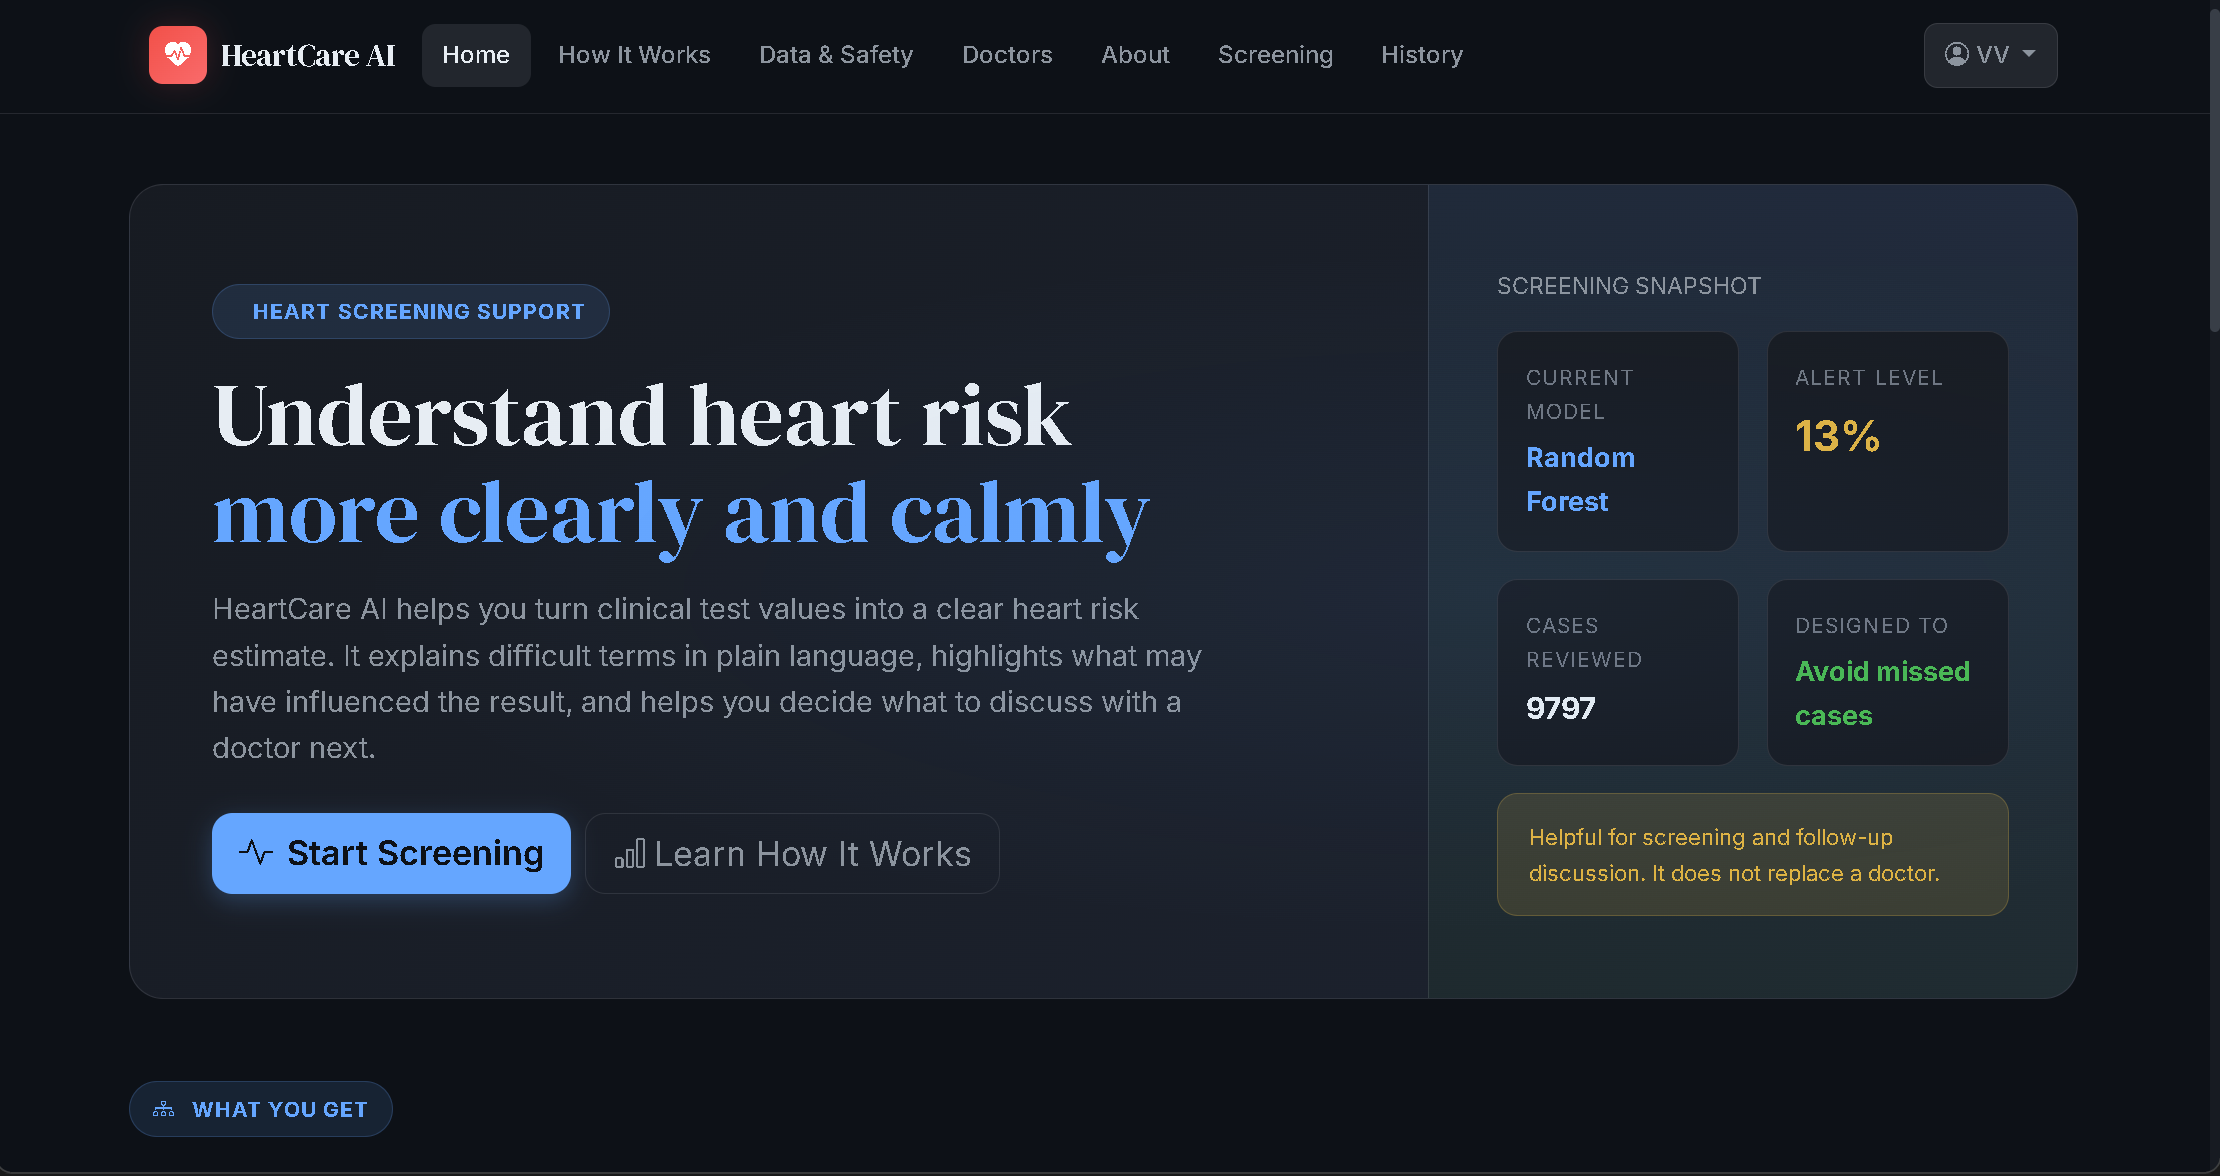
\includegraphics[width=\linewidth]{main_page.png}
    \caption{HeartCareAI main page showing the entry point for the web-based screening support application.}
    \label{fig:ui-main}
\end{figure}

\begin{figure}[!t]
    \centering
    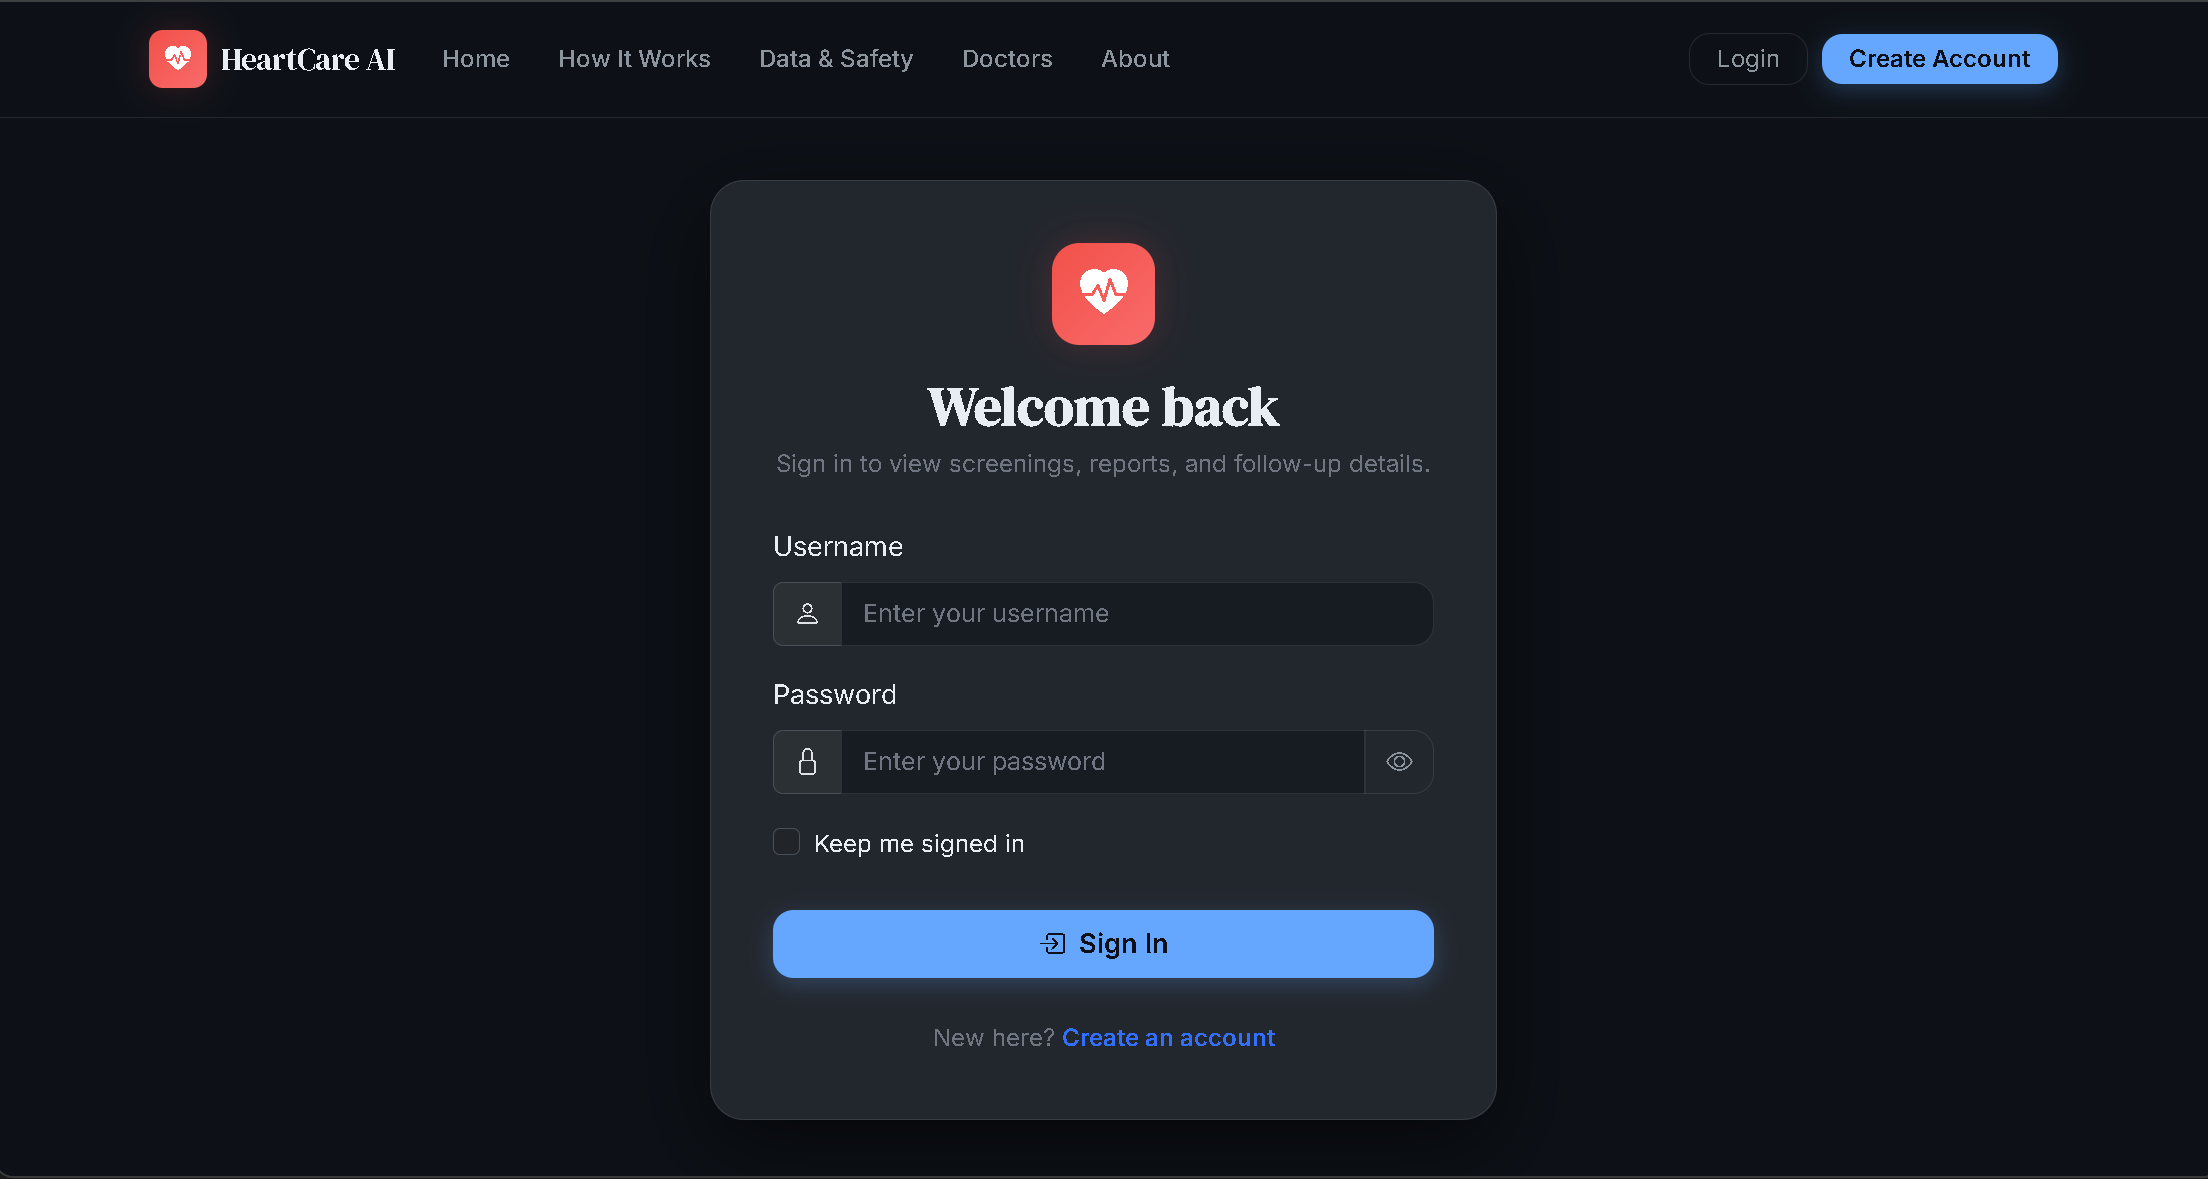
\includegraphics[width=\linewidth]{login_page_real.png}
    \caption{Login page controlling role-based access to the HeartCareAI workflow.}
    \label{fig:ui-login}
\end{figure}

\begin{figure}[!t]
    \centering
    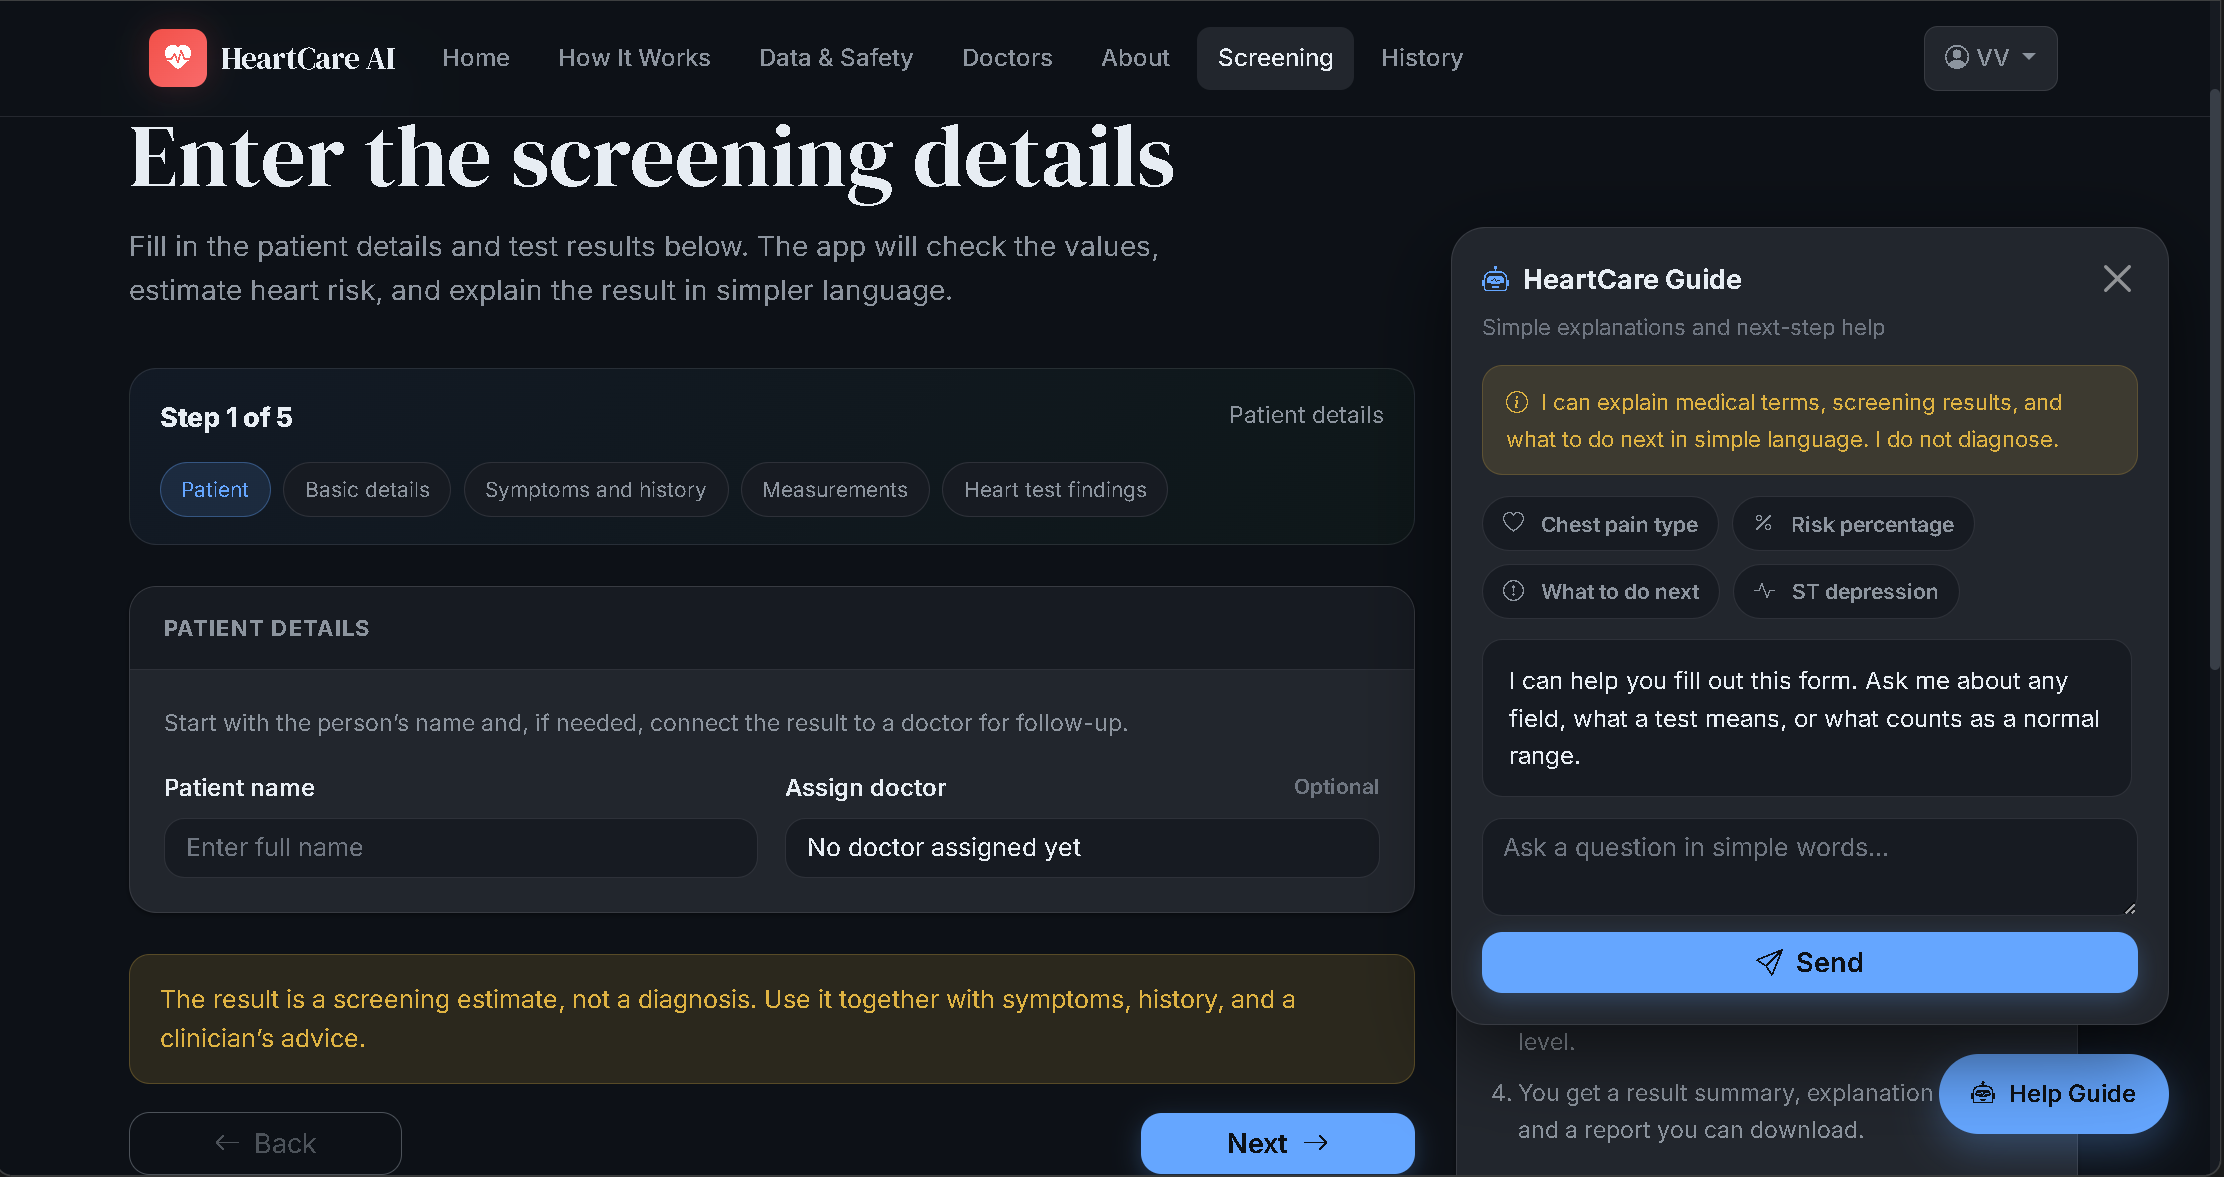
\includegraphics[width=\linewidth]{screening_page.png}
    \caption{Screening page used to collect validated clinical inputs for model inference.}
    \label{fig:ui-screening}
\end{figure}

\begin{figure}[!t]
    \centering
    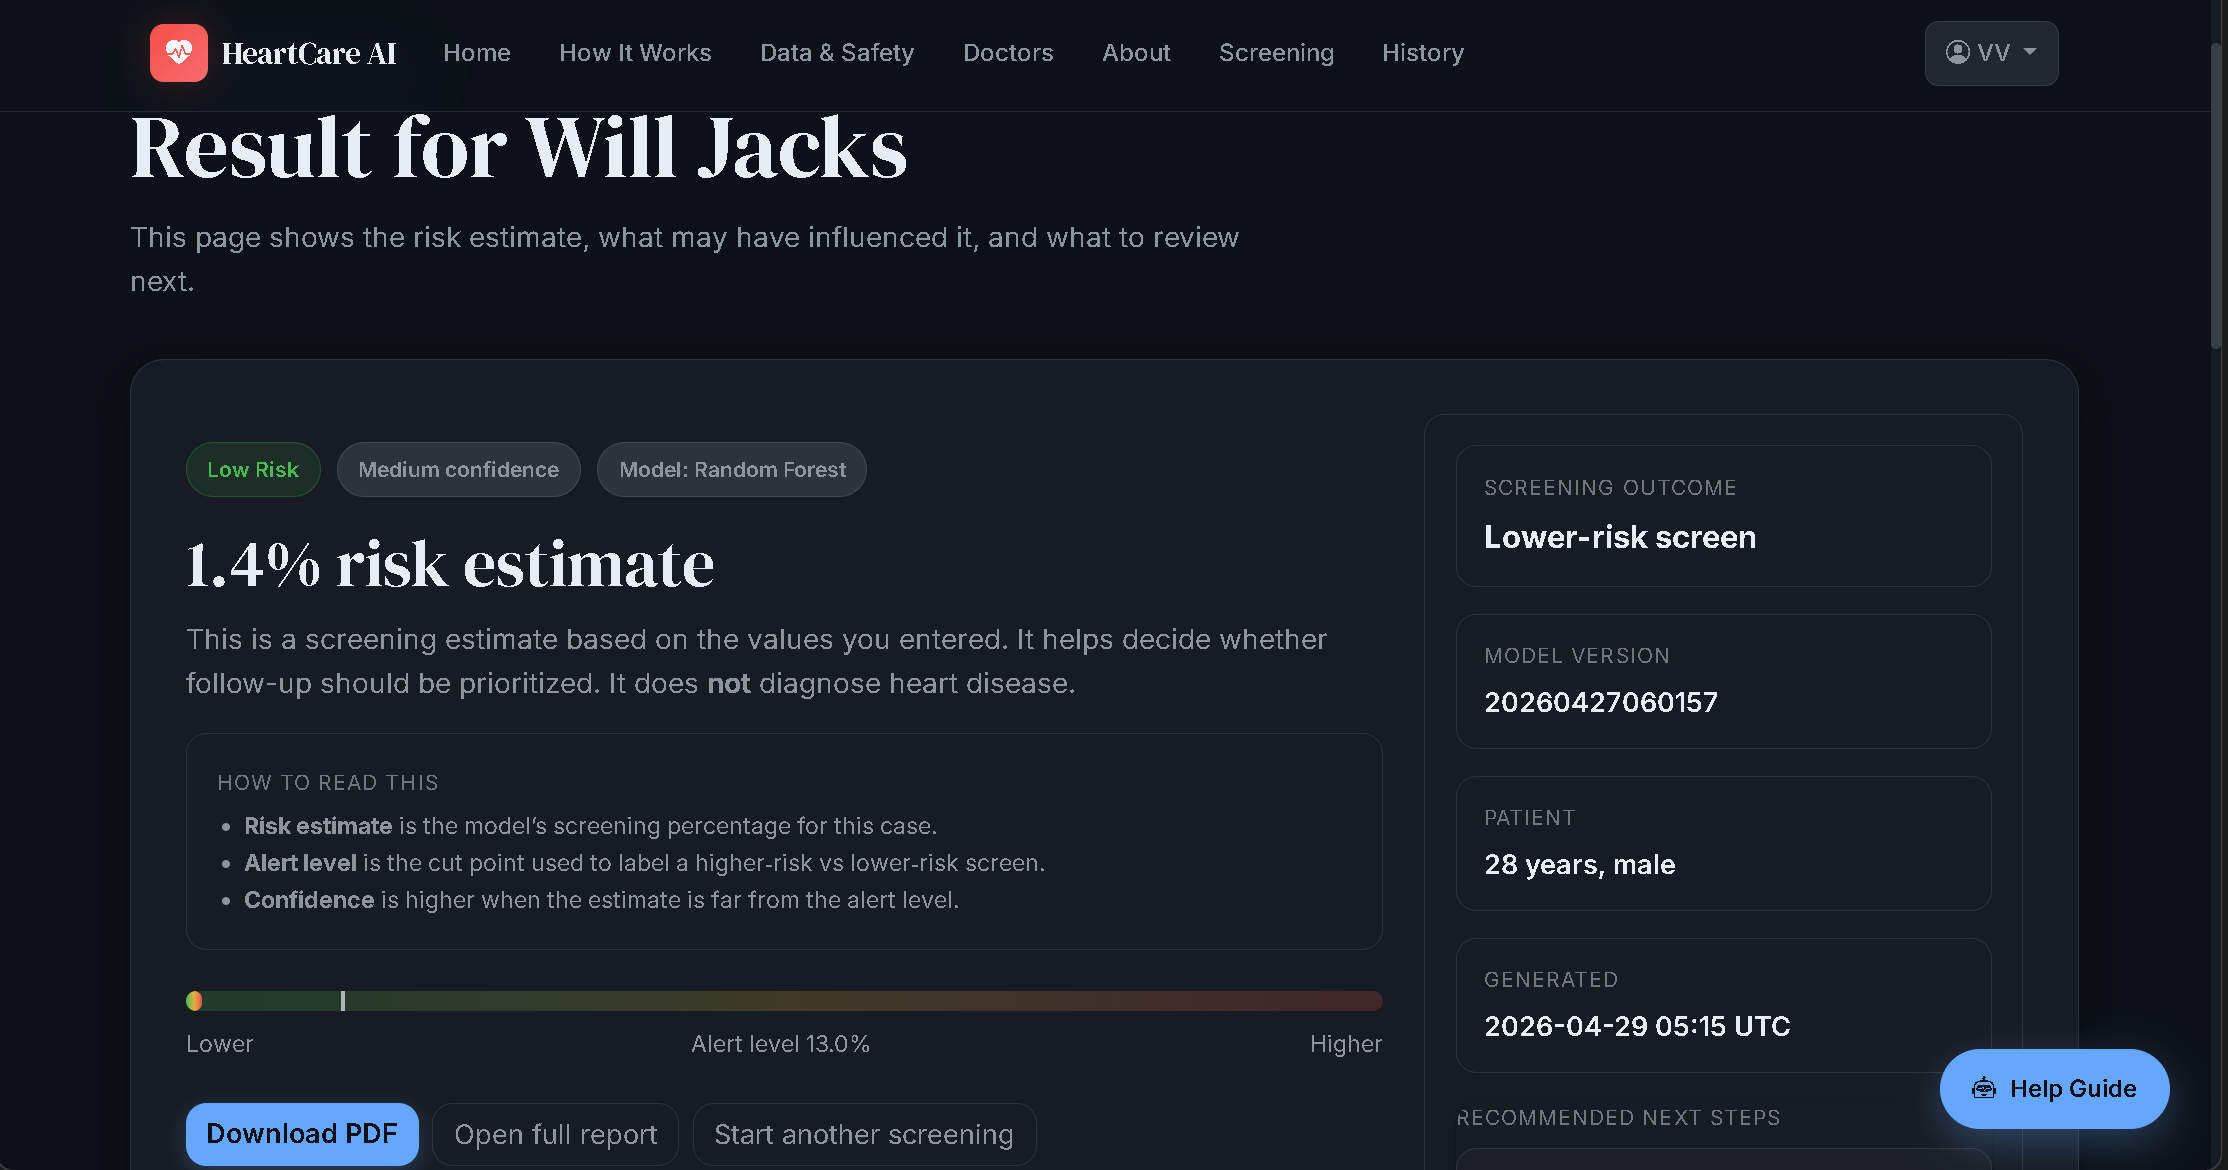
\includegraphics[width=\linewidth]{result_page.png}
    \caption{Prediction result page communicating the screening output to the user.}
    \label{fig:ui-result}
\end{figure}

\begin{figure}[!t]
    \centering
    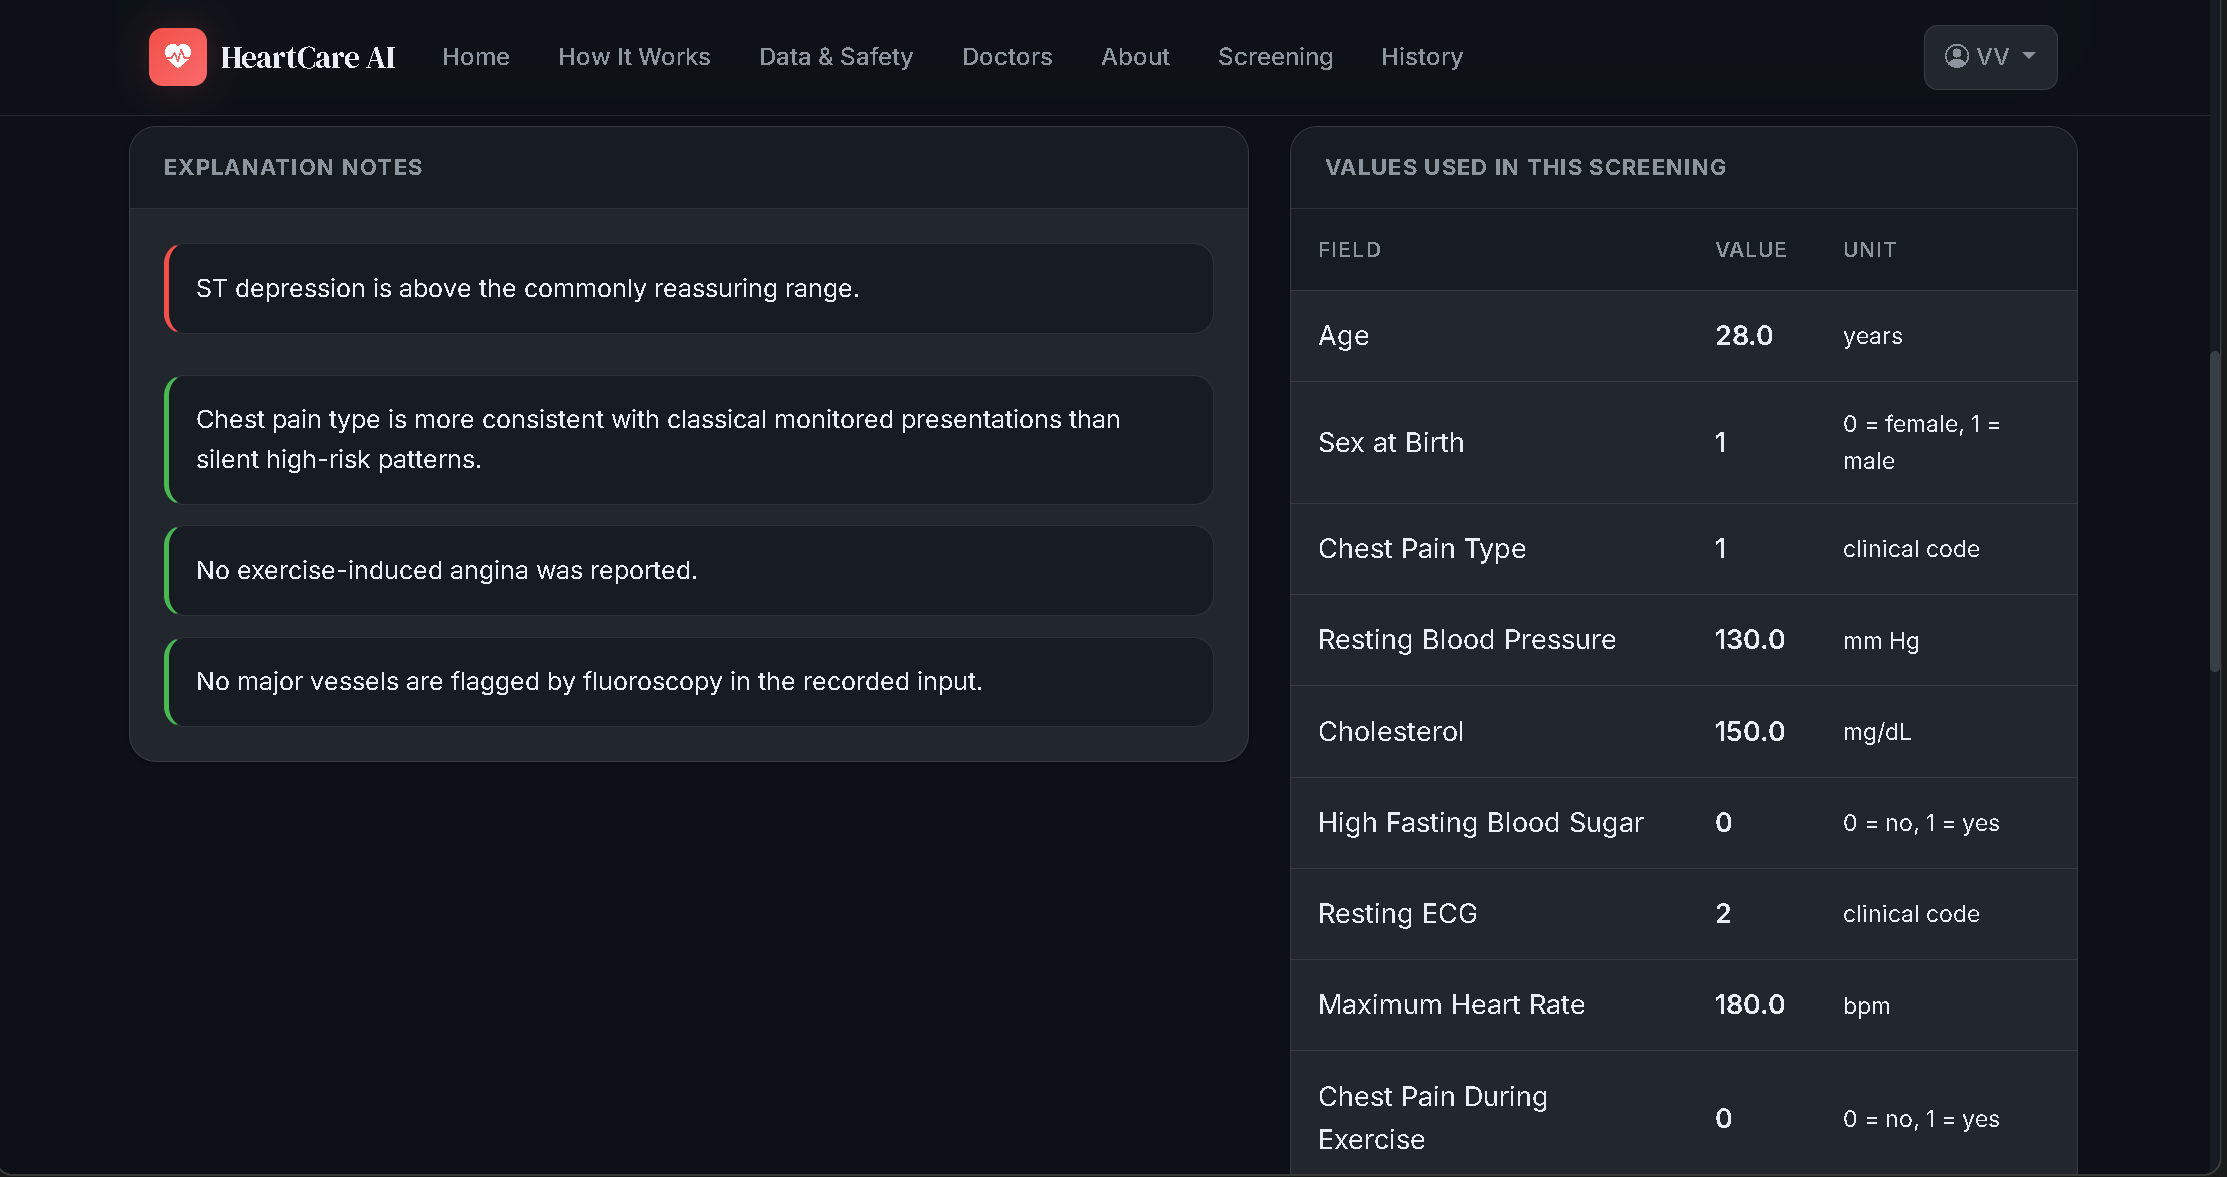
\includegraphics[width=\linewidth]{report_page_real.png}
    \caption{Report view preserving the prediction context for later review.}
    \label{fig:ui-report}
\end{figure}

\begin{figure}[!t]
    \centering
    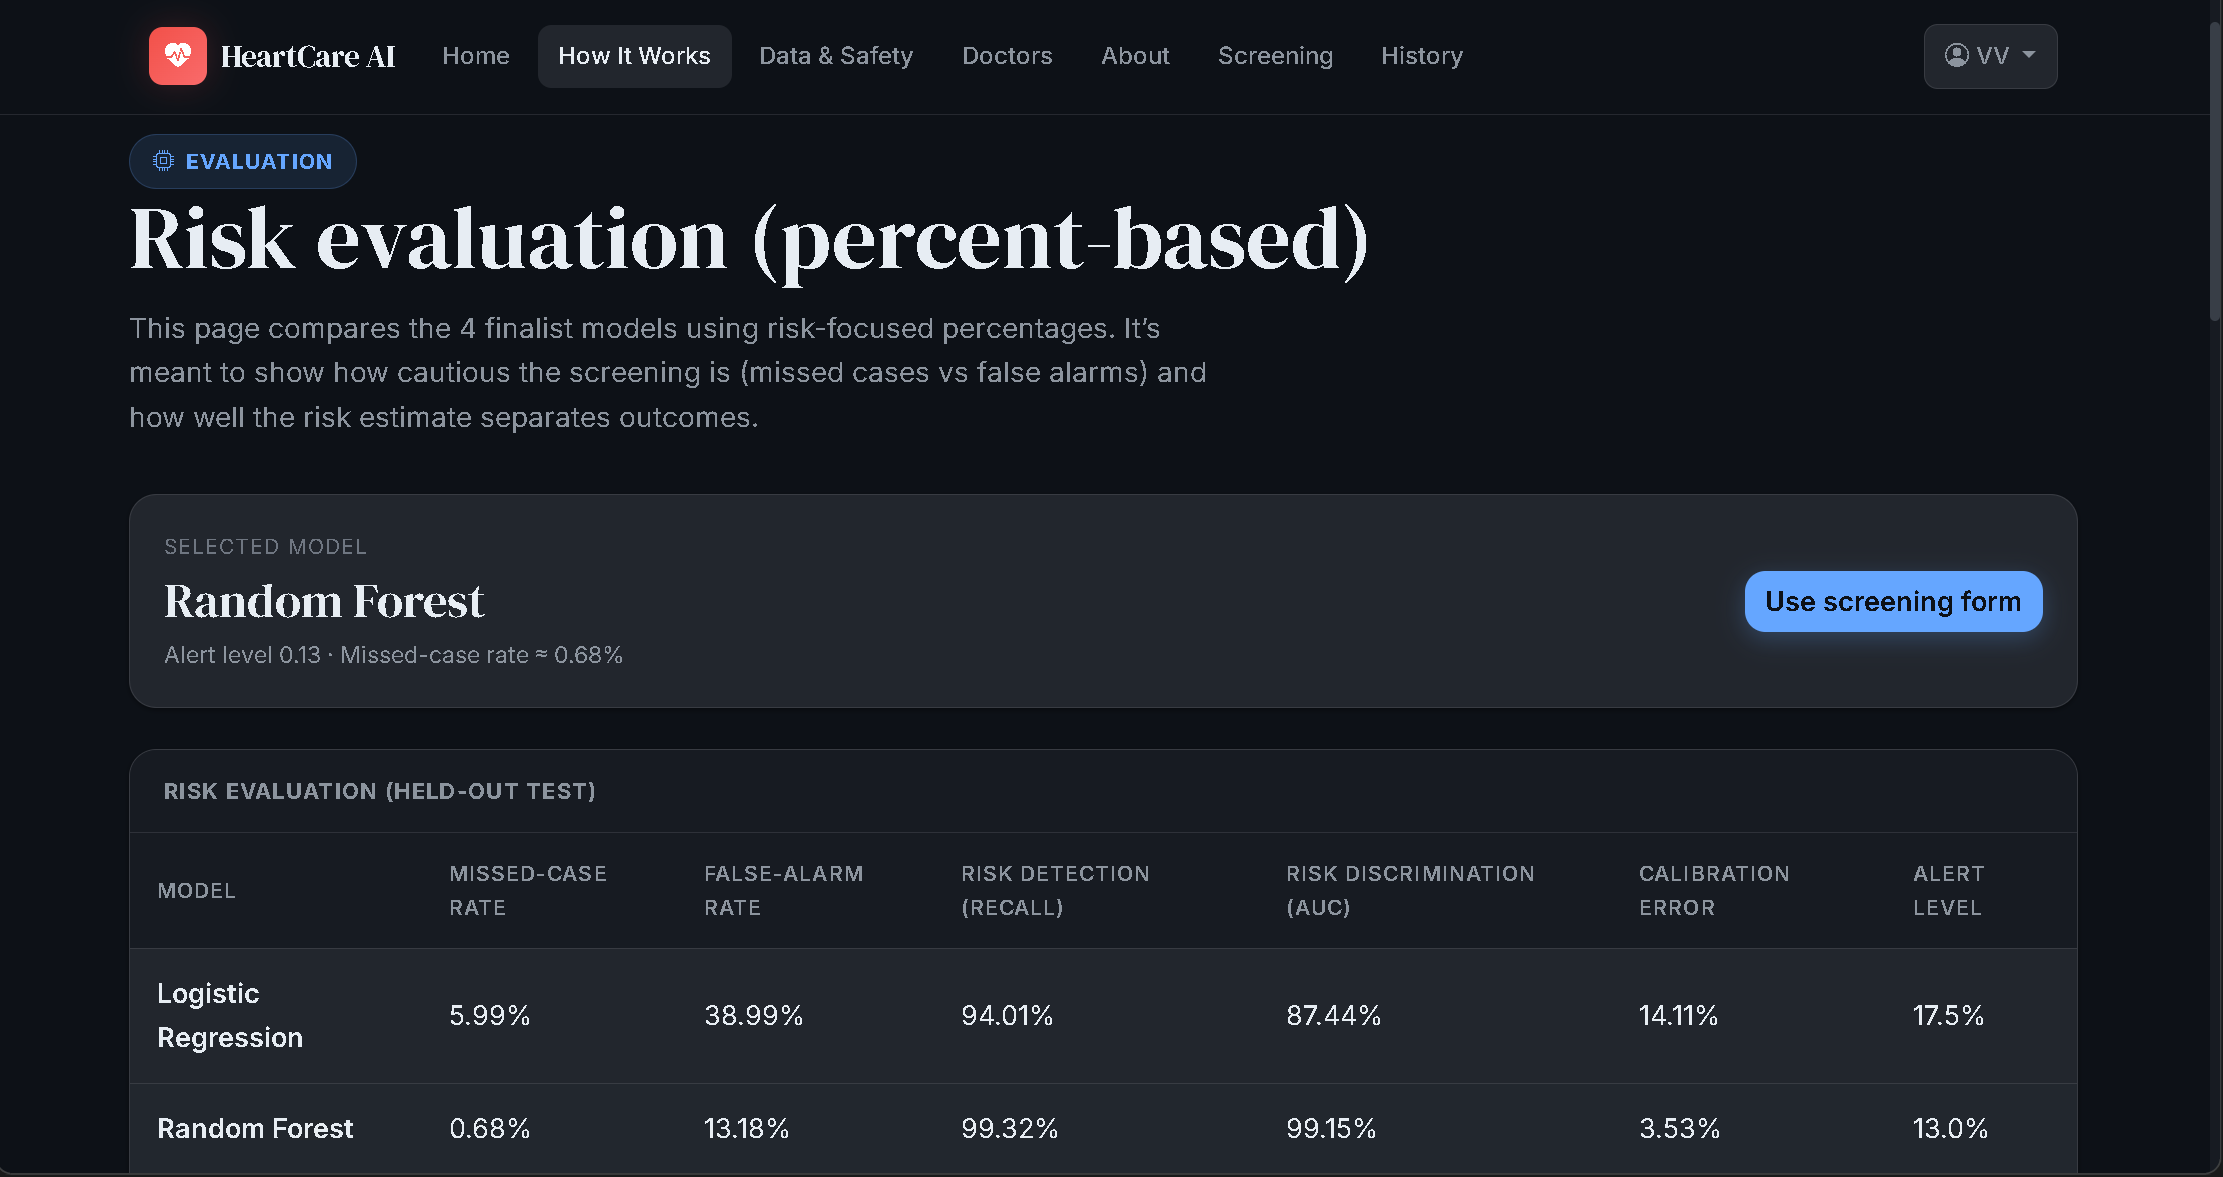
\includegraphics[width=\linewidth]{overview_page.png}
    \caption{Overview page used to summarize HeartCareAI workflow information.}
    \label{fig:ui-overview}
\end{figure}

\begin{figure}[!t]
    \centering
    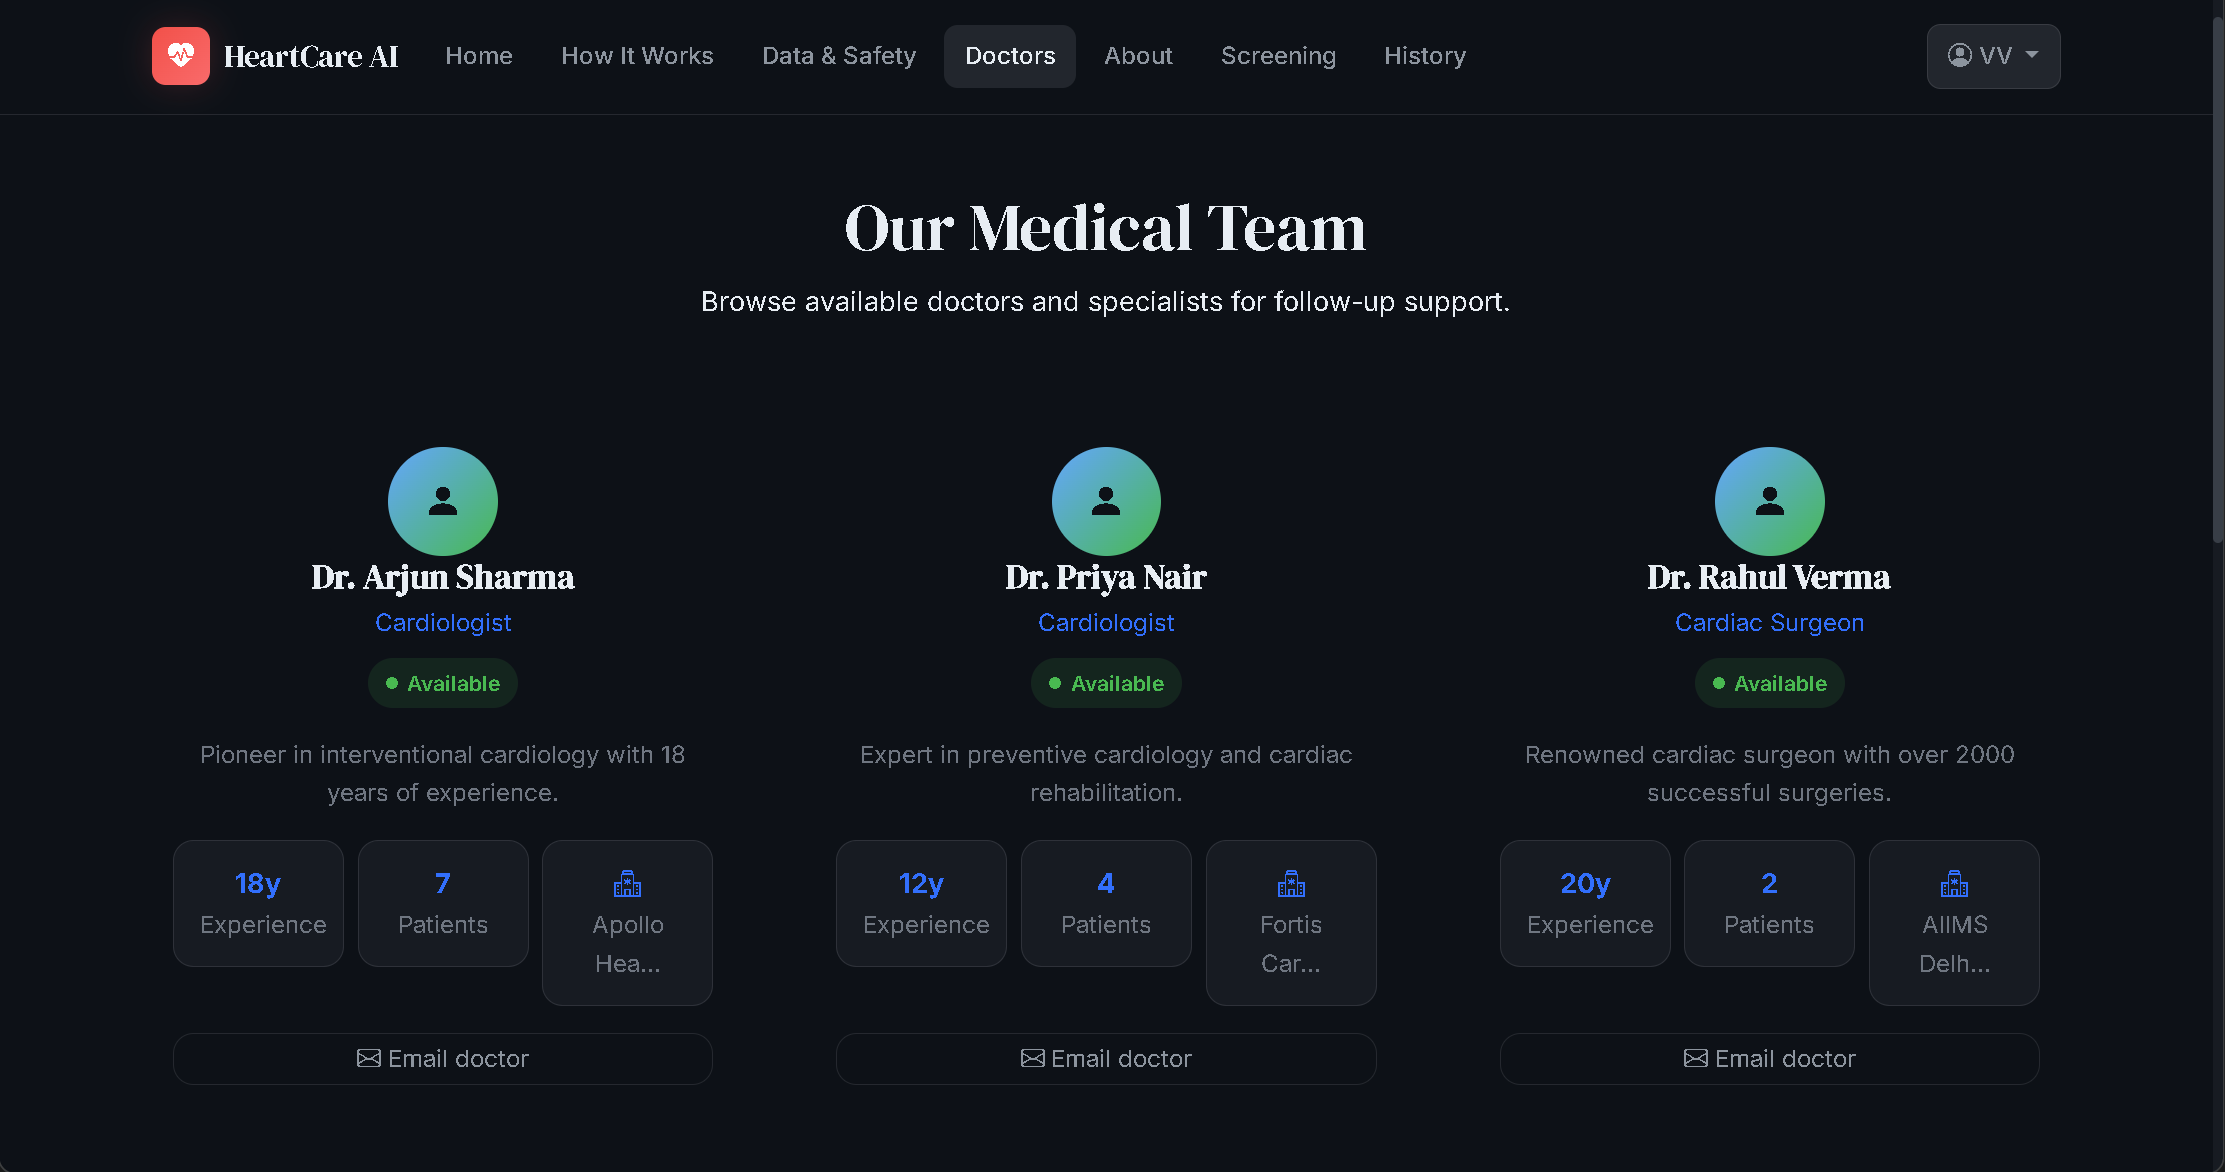
\includegraphics[width=\linewidth]{doctors_page.png}
    \caption{Doctor-facing page supporting review and monitoring in the application.}
    \label{fig:ui-doctors}
\end{figure}

\begin{figure}[!t]
    \centering
    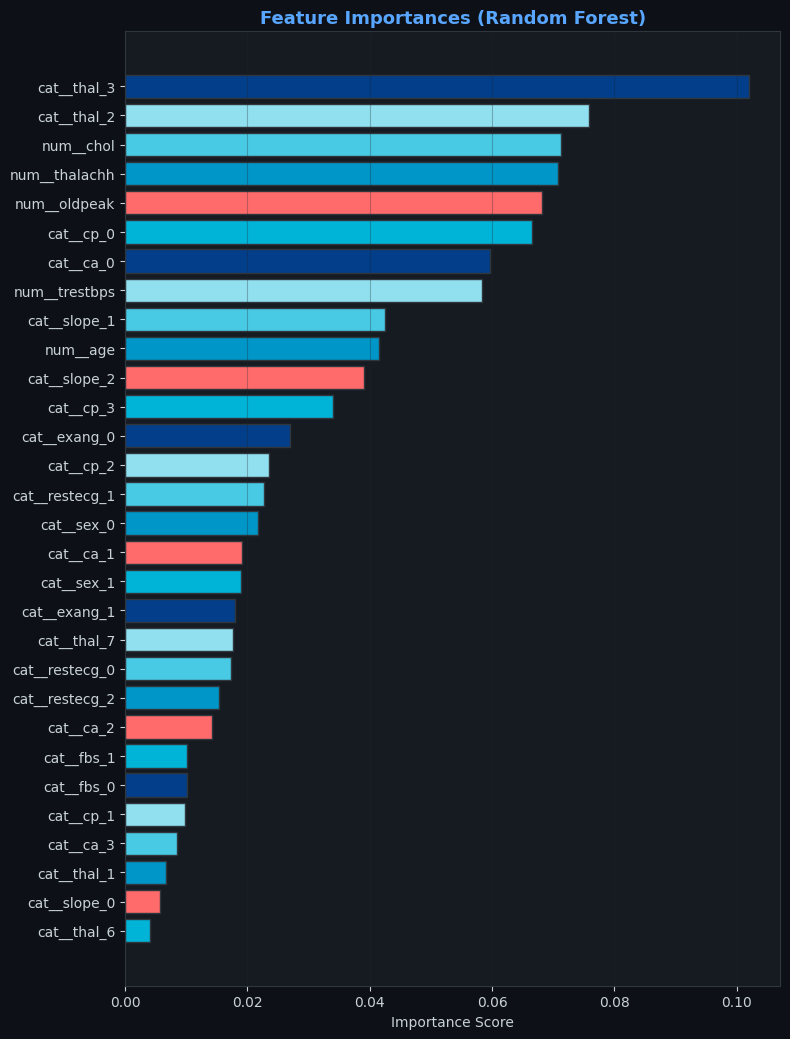
\includegraphics[width=\linewidth]{feature_importance.png}
    \caption{Feature importance visualization included in the model analysis pages.}
    \label{fig:importance}
\end{figure}

\begin{figure}[!t]
    \centering
    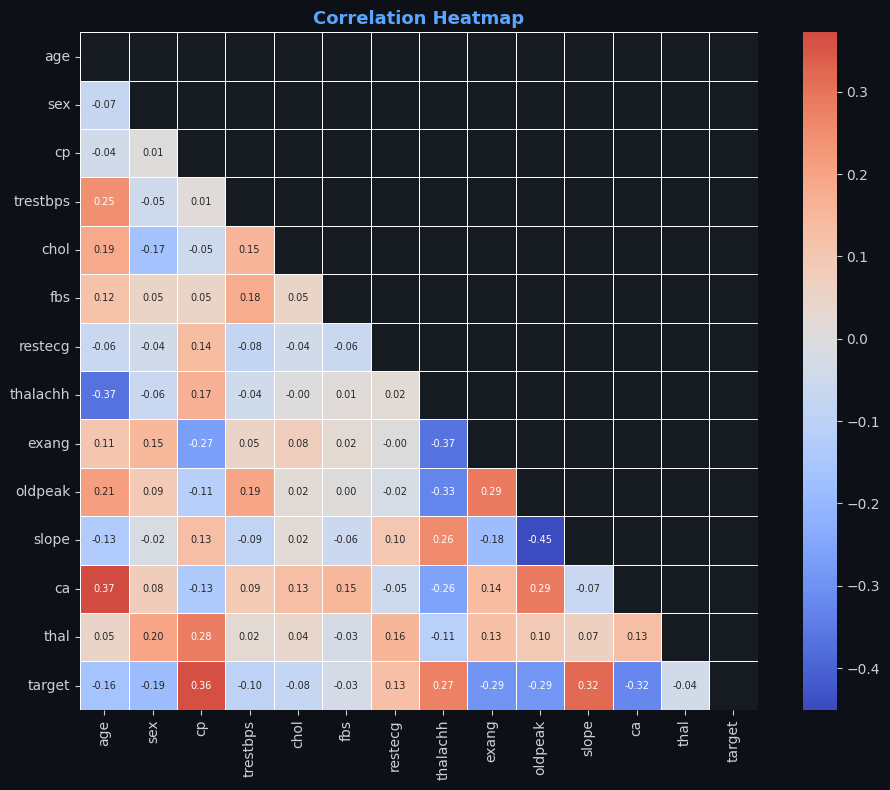
\includegraphics[width=\linewidth]{heatmap.png}
    \caption{Correlation heatmap used for exploratory data analysis.}
    \label{fig:heatmap}
\end{figure}

\section{Ethical, Safety, and Clinical Considerations}
HeartCareAI should be read as a screening support and educational research application. It is not a medical device, does not diagnose heart disease, and should not be used as a substitute for a qualified clinician. This boundary matters because a health-related prediction can affect anxiety, confidence, and the decision to seek or delay care.

Privacy and security are central concerns. Health-related inputs and prediction records should be protected through secure authentication, careful database access control, transport security, and limited exposure of sensitive information. The application should avoid displaying real patient identifiers in screenshots, reports, or demonstrations unless explicit permission and appropriate safeguards exist.

Bias is another important risk. A model trained on one dataset may perform differently across age groups, sex categories, regions, hospitals, measurement devices, and clinical workflows. Calibration, explainability, and audit logs can improve transparency, but they do not remove the need for external validation. Any future clinical deployment would require governance, prospective testing, human oversight, and compliance with applicable medical and data protection regulations.

\section{Limitations}
The current work has several limitations. First, the dataset may not represent all populations or clinical environments. Second, the very high reported performance may reflect dataset-specific patterns, preprocessing choices, or distributional similarity between training and evaluation records. Third, external hospital validation and prospective evaluation were not performed. Fourth, the application does not integrate with electronic health record standards such as FHIR. Fifth, the chatbot is informational and should not be used for diagnosis or treatment. Finally, the system requires deeper security review before production use, including stronger secret management, deployment hardening, access logging, and privacy controls.

\section{Future Work}
Future development should validate the model on multi-center datasets and compare performance across demographic and clinical subgroups. Explainability methods such as SHAP could help doctors inspect which features influenced a prediction, although explanations must be tested for usefulness and not treated as causal proof. The application can also be extended with FHIR-based data exchange, richer audit logs, model drift monitoring, calibration monitoring, clinician usability studies, and secure deployment practices. A long-term version should include governance for model updates so that changes in model artifacts are traceable and reviewable.

\section{Conclusion}
HeartCareAI demonstrates how a heart disease screening model can be embedded in a web-based workflow with role-aware access, input validation, calibrated probability output, reporting, visualization, and grounded chatbot support. The project shows that the practical value of machine learning in healthcare depends not only on classification metrics but also on the surrounding software, safety communication, traceability, and usability. The reported Random Forest performance is promising within the available project evaluation, but clinical use would require external validation, bias analysis, security hardening, and prospective review. In its present form, HeartCareAI should be treated as a research and educational screening-support system.

\bibliographystyle{IEEEtran}
\bibliography{references}

\end{document}
